\input{configuration}

\title{Lecture 31 --- Recovery: Repairing Inconsistent Data}

\author{Jeff Zarnett \\ \small \texttt{jzarnett@uwaterloo.ca}}
\institute{Department of Electrical and Computer Engineering \\
  University of Waterloo}
\date{\today}


\begin{document}

\begin{frame}
  \titlepage

 \end{frame}


\begin{frame}
\frametitle{Inconsistent data}

Inconsistent databases are a difficult problem for DB designers to deal with. 

As the definition of inconsistent suggests, one or more integrity constraints have been violated... 

\begin{center}
	
\includegraphics[width=0.4\textwidth]{images/breakingthelaw.jpg}
\end{center}


 \end{frame}


\begin{frame}
\frametitle{Inconsistent data}

One might conclude that queries on the database would be impossible or the answers meaningless.

\begin{center}
	
\includegraphics[width=0.5\textwidth]{images/jonsnow.jpg}
\end{center}

We do have things we can do...

\begin{center}
	
\includegraphics[width=0.4\textwidth]{images/hope.jpg}
\end{center}

\end{frame}


\begin{frame}
\frametitle{Be Consistent...}

We say a database $D$ is \alert{consistent} if $D$ satisfies the set of integrity constraints $C$.

If any of these constraints are not met, the database is \alert{inconsistent}.

When there are inconsistencies whereby there are multiple tuples reflecting the same real-world entity, we name that a \alert{cluster}.


\end{frame}

\begin{frame}
\frametitle{How Did We Get Here?}

The obvious source of how databases may become inconsistent is: errors. 

Data can be entered that violates integrity constraints. 

That can happen if the database was implemented without certain important integrity constraints (e.g., foreign keys) added, or a new rule is being added. 

\end{frame}

\begin{frame}
\frametitle{How Did We Get Here?}

It can also happen because database integrity constraints can be turned off, or perhaps because the database engine just does not enforce those constraints. 

\begin{center}
	
\includegraphics[width=0.4\textwidth]{images/youwhat.jpg}
\end{center}

So in all cases, the inconsistency was added in error. 

\end{frame}


\begin{frame}
\frametitle{Strictness isn't Everything}

However, it is not the case, that by simply relying on error-detection and rule enforcement, we can be certain that no inconsistencies will ever arise. 

\begin{center}
	
\includegraphics[width=0.4\textwidth]{images/mistakes.jpg}
\end{center}

One way it could be inconsistent is from data warehousing; when data is imported from various sources and may need cleaning before storing. 

\begin{center}
	
\includegraphics[width=0.4\textwidth]{images/peaceorder.jpg}
\end{center}
\hfill ``Soon peace and order will be restored throughout the galaxy.''

One way it could be inconsistent is from data warehousing; when data is imported from various sources and may need cleaning before storing. 

\end{frame}


\begin{frame}
\frametitle{Strictness isn't Everything}

The second is database integration: when some data is stored across many databases stitched together.

It is possible that integrity checking may simply be too costly from a performance standpoint.

Finally, we might sometimes choose to allow a temporary inconsistency.

\end{frame}


\begin{frame}
\frametitle{Moving Forward with Inconsistencies}

We would like the answer from a query against an inconsistent database to be the same as that of the consistent database. 

At the very least, we are interested in getting a consistent answer to a query, even in the presence of inconsistent data. 

We may also be interested in repairing the database, so that the inconsistencies may be removed entirely.

\end{frame}


\begin{frame}
\frametitle{Fix It!}

When presented with an inconsistent database, we might be able to repair it. 

\begin{center}
	
\includegraphics[width=0.3\textwidth]{images/flextape.png}
\end{center}

The nature of the repair will obviously be context-dependent. 

\end{frame}

\begin{frame}
\frametitle{Fix It!}

The basic definition of a repair $D'$ of a database $D$ is that $D'$ is a modification of $D$ such that $D'$ meets the constraint set $C$.

\begin{center}
	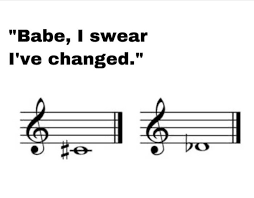
\includegraphics[width=0.5\textwidth]{images/changed.png}
\end{center}


\end{frame}


\begin{frame}
\frametitle{Basic Principles of Repairs}

There are infinitely many such database repairs that can be performed. 

\begin{center}
	
\includegraphics[width=0.25\textwidth]{images/thanos1.jpeg}
\end{center}


We add a further restriction; that the new database $D'$ is changed only minimally from the original $D$.

\begin{center}
	
\includegraphics[width=0.25\textwidth]{images/thanos2.jpg}
\end{center}

\end{frame}

\begin{frame}
\frametitle{Basic Principles of Repairs}
Making the minimal set of changes necessary to meet all constraints $C$ is nice.


If a database is consistent, then the minimal repair is to do nothing ($D' = D$). 

Furthermore, we will always be able to find a repair to the database.

\end{frame}




\begin{frame}
\frametitle{Minimal = Best?}

With that in mind, it is sometimes undesirable to make the minimal set of changes, because that may simply be deletion of the offending tuple(s). 

\begin{center}
	
\includegraphics[width=0.7\textwidth]{images/indy.jpg}
\end{center}

\end{frame}

\begin{frame}
\frametitle{Minimal = Best?}

While deletion may bring the database into a consistent state, it also may mean data loss, and that is generally not our first choice. 

We are therefore forced to keep our minds open to repairs that are not the minimal set of changes, but as minimal as possible without data loss.


\end{frame}


\begin{frame}
\frametitle{Example Data: Salaries}


\begin{table}[h]\begin{center}
        \begin{tabular}{r | c  c} 
					salaries & employee\_name & salary \\ \hline
	           		 & J. Page  & 50 000 \\ 
	         		 & J. Page  & 80 000 \\ 
					 & V. Smith & 35 000 \\ 
					 & M. Stowe & 75 000 \\ 
        \end{tabular}
\end{center}\end{table}

The constraint is violated for the user ``J. Page"; he or she has two salaries.

\begin{center}
	
\includegraphics[width=0.3\textwidth]{images/cra.jpg}
\end{center}

\end{frame}

\begin{frame}
\frametitle{Fixing It}

There are two possible repairs that we can make to this relation:

\begin{table}[h]\begin{center}
        \begin{tabular}{r | c  c} 
					salaries & employee\_name & salary \\ \hline
	         		 & J. Page  & 80 000 \\ 
					 & V. Smith & 35 000 \\ 
					 & M. Stowe & 75 000 \\ 
        \end{tabular}
\end{center}\end{table}

\begin{table}[h]\begin{center}
        \begin{tabular}{r | c  c} 
					salaries & employee\_name & salary \\ \hline
	           		 & J. Page  & 50 000 \\ 
					 & V. Smith & 35 000 \\ 
					 & M. Stowe & 75 000 \\ 
        \end{tabular}
\end{center}\end{table}

\end{frame}


\begin{frame}
\frametitle{Making the Repair}

In either case, we return to a consistent database, because the sole constraint is now correctly enforced.

Throwing away all tuples that participate in the violation results in data loss.

Doing so would not be the minimal set of changes to the system - throwing away one would be enough.

\end{frame}


\begin{frame}
\frametitle{Performing More Complex Repairs}

There are some specific circumstances under which we might face infinitely many or infeasibly many repairs. 

How to repair a string such that it is unique in the relation? 


\end{frame}


\begin{frame}
\frametitle{Performing More Complex Repairs}

The number of possible strings which meet this condition is infinite (though it may be constrained from infinite to infeasible by limiting the length attribute. 


\end{frame}


\begin{frame}
\frametitle{Performing More Complex Repairs}

Under those circumstances, insert a \texttt{null} into that attribute.

But the relational model may forbid a null in this attribute...


\end{frame}


\begin{frame}
\frametitle{Specifying Repairs with Annotations}

The pressing question now is what repairs to perform. 

Annotated logic, specifically, \alert{Annotated Predicate Calculus} provides a method.

In APC, we annotate database atoms (components) with true ($t$), false ($f$), contradictory ($\top$), and unknown ($\bot$).


\end{frame}

\begin{frame}
\frametitle{Truth Values}

The truth values in the lattice are as follows:

\begin{itemize}
\item \textit{Basic Values}: $t$, $f$, $\top$, and $\bot$.
\item \textit{Database Values:} $t_d$, $f_d$.
\item \textit{Constraint Values:} $t_c$, $f_c$ (also $t$ and $f$).
\item \textit{Advisory Values:} $t_a$, $f_a$.
\end{itemize}



\end{frame}

\begin{frame}
\frametitle{Truth Lattice}

\begin{figure}[!h]
  \centering \includegraphics[width=0.7\textwidth]{images/TruthLattice.pdf}
\end{figure}


\end{frame}

\begin{frame}
\frametitle{Truth Lattice Examples}

In the simplest case, if we have something true in the database ($t_d$), and true in the constraints ($t_c$), then we can move simply to true ($t$), without problem. 

If we find something true in the database ($t_d$) yet false according to the constraints ($f_c$), then we can move to $f_a$ - suspected false. 

If we have an irresolvable conflict, for example, finding one thing certainly true and the other certainly false, we move to $\top$.

\end{frame}

\begin{frame}
\frametitle{Truth Lattice Examples}

We consider data to be fallible, but constraints to be correct.

Thus, if an atom gets both $t_d$ and $f_c$, we will resolve that conflict as $f_a$; 
 
 At the end of the evaluation, in order to repair the database, things we believe to 
be false will be removed.

Things we believe to be true will be inserted into the database.

\end{frame}

\begin{frame}
\frametitle{Truth Lattice Guides Us}

If we apply this principle to an inconsistent database, then the results we will get will indicate our best course of action. 

The results received will simply be a set of advice: add this; delete that.

A program can use the set of advisory values to repair the database.


\end{frame}


\begin{frame}
\frametitle{Specifying Repairs with Logic Programs}

We can also make use of a logic program alone to find repairs.

Consider a logic program with exceptions to these rules. The exceptions naturally have a higher priority than the rules.

Most of the time, when we repair a database, most data is preserved, but some tuples will be removed. 

\end{frame}


\begin{frame}
\frametitle{Specifying Repairs with Logic Programs}

We can combine the appropriate logic program with the idea of logical consequence, and use this to compute repairs.

To do so, we must find atoms true in every answer set of the program. 

This approach functions for all first-order queries, but it may be impractical because the size can quickly get out of hand.

\end{frame}

\begin{frame}
\frametitle{Aggregate Queries}

In some circumstances, the answers to aggregate queries are easy. 

If we look once again at the examples of salary data, and we want to select the minimum salary. 

V. Smith's salary of \$35~000 is returned under all possible repairs. 

\end{frame}

\begin{frame}
\frametitle{Aggregate Queries}

If instead we sought the maximum, both repairs offer different answers. 

Instead, we return an interval where the minimum is the lower bound from all possible repairs, and the maximum is the upper bound. 


\begin{center}
	
\includegraphics[width=0.3\textwidth]{images/uncertainty.jpg}
\end{center}

In this example, we consider [75~000,~80~000] to be a consistent answer to the aggregation query.

\end{frame}

\begin{frame}
\frametitle{Open Issues}

The major open issue they identify is how to deal with global constraints in a composite database system. 

It is unclear what a consistent answer is in such a context, and similarly unclear what a repair means.

Another suggestion is to move this into the database management system. 

This would allow soft integrity constraints (not explicitly enforced), and different users could have different constraints.

\end{frame}

\begin{frame}
\frametitle{Query Transformation}

Another option: query transformation. 

Instead of modifying the database and then running the query on the new database, we transform the query and run it against the unaltered database. 

We change the query such that for every possible database $D'$ the answers to said query is equal to the consistent answers.


\end{frame}

\begin{frame}
\frametitle{Gross...?}

We will consider first-order queries, and only universal integrity constraints. 

We iterate the transformation of the query by conjoining the \alert{residues} to the results of the query. 

We continue until the query in iteration $n$ is identical to that in $(n-1)$.

If there are no residues, then the query needs no alterations.


\end{frame}

\begin{frame}
\frametitle{Residues}

But what is a residue? Consider the following example constraint set:
\begin{center}
$C = \{\forall x.[R(x) \bigvee \neg P(x) \bigvee \neg Q(x)], \forall x.[P(x) \bigvee \neg Q(x)] \}$ 
\end{center}

We will focus on $Q(x)$ as our target query. 

\end{frame}

\begin{frame}
\frametitle{Residues}

The residue of $Q(x)$ with respect to the first constraint is $R(x) \bigvee \neg P(x)$; if the constraint and $Q(x)$ are true, then the residue must also be. 

The residue with respect to the second constraint is $P(x)$. 

Finally, the $\neg Q(x)$ component does not have any residues, because the integrity constraints do not constrain it. 

Here, they don't, but in theory, the residues might themselves have residues.

\end{frame}

\begin{frame}
\frametitle{Not just the Query}

Instead of running the query $Q(x)$, we ask $Q(x)$ together with each of its residues. 

More formally, it is $Q(x)$ is logically AND-ed with each residue, as follows:

\begin{center}
$Q(x) \bigwedge (R(x) \bigvee \neg P(x)) \bigwedge P(x)$
\end{center}

The effect of this altered query is to return only the answers to $Q(x)$ for which the constraints hold.

\end{frame}


\begin{frame}
\frametitle{Salaries Again}

Looking at the previous example of salaries.

The modified query will ask for the names and salaries of all employees ($Q(x)$) where there is only one entry in the relation for that user.

This will return two tuples (V. Smith and M. Stowe). 

No data will be returned for tuples where there is a violation (J. Page), so no data is shown reflecting our uncertainty about his salary.


\end{frame}

\begin{frame}
\frametitle{Algorithmic Validity}

The algorithm hangs on soundness, completeness, and termination.

The soundness principle is the most obvious - every answer to the altered query must be a consistent answer to the original.

Completeness is necessary so that every consistent answer to the original query appears as an answer to the transformed one. 

Termination means that there will always be a reachable point at which we may stop the query modification iterations.

\end{frame}



\begin{frame}
\frametitle{Problems with This Approach}

If we apply query transformation to the table of salaries, this will certainly return only the consistent answers from the database (V. Smith and M. Stowe). 

Neither of the tuples for J. Page will be returned, because they are inconsistent. 

This may sometimes be desirable, if we do not wish to report information we are uncertain about. 

\end{frame}



\begin{frame}
\frametitle{Problems with This Approach}

However, under some circumstances, it is probably undesirable to simply ignore the tuples that are inconsistent. 

\begin{center}
	
\includegraphics[width=0.3\textwidth]{images/forgetting.jpg}
\end{center}

Surely J. Page would prefer that the discrepancy in pay be alerted to someone!


\end{frame}

\begin{frame}
\frametitle{Can't Rewrite Them All}

Query rewriting fails in the case of a disjunctive or existential queries, but only fails in the completeness category. 

The methodology is intended only to handle universal integrity constrains, and therefore existential qualifiers present problems. 


\end{frame}

\begin{frame}
\frametitle{Can't Rewrite Them All}

Existential qualifiers may lead to co-NP-completeness, and computational feasibility issues prevent the fulfillment of the completeness criterion. 

\begin{center}
	
\includegraphics[width=0.3\textwidth]{images/migraine.jpg}
\end{center}


\end{frame}


\end{document}

